\chapter{Implementación}\label{cap4}

\section{Tecnologías utilizadas}
%-------------------------------------------------------------------------------
\subsection{Base de datos relacional}\label{sec-bd-r}
Una base de datos relaciones es una colección de tablas relacionadas entre sí. La colección de tablas se describe a sí misma en cuanto a que el significado de los datos contenidos pertenecen a un mismo ámbito\cite{DataBaseConcepts}.\\
Una base de datos es administrada mediante un Sistema Administrador de Bases de Datos (DBMS por sus siglas en inglés), un DBMS es un programa de computadora usado para crear, procesas y administrar bases de datos. El DBMS recibe peticiones en lenguaje SQL (como se describe más adelante) y traduce esas peticiones a acciones dentro de la base de datos\cite{DataBaseConcepts}.\\
Para el desarrollo del proyecto AutoSA se han usado los siguientes conceptos:
\begin{enumerate}
	\item \textbf{Tabla}: una tabla es un conjunto de renglones (registros) y columnas (atributos) que cumple con las siguientes características\cite{DataBaseConcepts}:
	\begin{enumerate}
		\item Los renglones contienen unicamente datos relacionados con la tabla.
		\item Las entradas de una columna contienen un solo valor.
		\item Todas las entradas de una columna son del mismo tipo.
		\item Las columnas tienen un nombre único dentro de la tabla.
		\item El orden de las columnas y los renglones no es relevante.
		\item No contiene dos renglones idénticos.
	\end{enumerate}
	\item \textbf{Vista}: es una tabla derivada de una consulta de otras tablas, estas tablas pueden ser tablas de la base de datos o vistas definidas previamente. Una vista es considerada como tabla virtual porque no necesariamente existe físicamente a diferencia de una tabla de la base cuyas tuplas siempre están almacenadas físicamente en la base de datos\cite{FundamentalsOfDBSystems}.
	\item \textbf{Llave primaria}: es el conjunto de columnas que identifican de manera unívoca a cada renglón de la tabla.\cite{DataBaseConcepts}
	\item \textbf{Llave foránea}: define la relación de una tabla, \textbf{A}, hacia otra \textbf{B} y satisface las siguientes condiciones\cite{FundamentalsOfDBSystems, DataBaseConcepts}:
	\begin{enumerate}
		\item Los atributos de las tablas \textbf{A} y \textbf{B} son del mismo tipo y se corresponden uno a uno.
		\item Los atributos en la tabla \textbf{B} son exactamente los mismos de la llave primaria de la tabla \textbf{B}.
	\end{enumerate}
	\item \textbf{Restricción de integridad}: son reglas que se utilizan para asegurar que cambios en los datos de las tablas no causen inconsistencia en la información\cite{DatabaseSystemConcepts}.
	\begin{enumerate}
		\item NOT NULL: indica que el valor del atributo no puede ser nulo\cite{FundamentosSistemasBasesDatos}.
	\end{enumerate}
	\item \textbf{Índice}: es una estructura auxiliar para agilizar la obtención de registros. Los índices proveen rutas de acceso alternativo a los registros de la base de datos sin afectar la colocación física de los registros\cite{FundamentalsOfDBSystems}.
	\item \textbf{Lenguaje Estructurado de Consulta}\label{sec-sql}: del inglés Structured Query Language (SQL), fue desarrollado por IBM\textsuperscript{\textcopyright} al final de los años 70, es un lenguaje de datos orientado a texto, ha sido avalado por el Instituto Nacional de Estándares Americanos (ANSI por sus siglas en inglés) dando así los estándares ANSI para SQL, principalmente para este trabajo el estándar ANSI-92 o SQL-92.
	\item \textbf{Lenguaje de Definición de Datos}: DDL por sus siglas en inglés, es un lenguaje de SQL cuya función es describir la creación de estructuras tales como tablas, índices y restricciones, entre otras\cite{DataBaseConcepts}.
	\item \textbf{Lenguaje de Modelado de Datos}: DML por sus siglas en inglés, es un lenguaje de SQL cuya función es describir la modificación de datos, es decir, sentencias de inserción, borrado y actualización de datos\cite{DataBaseConcepts}.  
\end{enumerate}

%-------------------------------------------------------------------------------
\subsection{Java}\label{sec-java}

El lenguaje de programación Java fue creado en 1991 por James Gosling, Patrick Naughton, Chris Warth, Ed Frank y Mike Sheridan en 1991 bajo el nombre ``Oak'' y en 1995 cambiaron el nombre a Java. El lenguaje Java está basado en los lenguajes de programación C, de donde deriva su sintaxis y de C++, que se toma como base para las características del paradigma orientado a objetos. Java es un lenguaje orientado a objetos, estáticamente tipado y multiplataforma\cite{JavaCompleteReference, WellGroundedJavaDeveloper}.\\
El concepto de Java tiene varios componentes, para efectos de este proyecto se mencionarán los siguientes\cite{JavaCompleteReference, WellGroundedJavaDeveloper}:
\begin{enumerate}
	\item Lenguaje de programación Java: previamente descrito, es un lenguaje multiplataforma, estáticamente tipado y orientado a objetos.
	\item Máquina Virtual de Java: JVM por sus siglas en inglés, es el sistema de ejecución en tiempo real de Java\footnote{\textcolor{red}{Karla, \textbf{Sistema de ejecución en tiempo real de Java} fue lo que me pareció más correcto para traducir ``Java run-time system'' ¿qué opinas, sabes una traducción mejor?}}.
	\item Bytecode: es el nombre que recibe el conjunto optimizado de instrucciones diseñadas para ser ejecutadas en la JVM.
	\item Paquete de Desarrollo de Java JDK (Java Development Kit): es el conjunto de herramientas utilizadas para el desarrollo de software para la máquina virtual de Java.
	\item Ambiente de Ejecución de Java JRE (Java Runtime Environment): es la herramienta encargada de la creación y administración de instancias de la máquina virtual de Java.
\end{enumerate}

\subsubsection{Java Data Base Controller}\label{sec-jdbc}
El controlador de base de datos de Java (JDBC por sus siglas en inglés) es un conjunto de APIs\footnote{API viene del inglés ``Application Programming Interface'' este concepto es utilizado para denotar los métodos que proporciona una biblioteca.} que simplifica la conexión a bases de datos relacionales, cabe mencionar que por medio del API JDBC también se puede tener acceso a otras fuentes de datos como los son hojas cálculo, archivos de texto plano o bases de datos no relacionales\cite{JDBCRecipes, BeginingJava8APIs}.

%-------------------------------------------------------------------------------
\subsection{Spring}\label{sec-spring}
El marco de trabajo Spring es descrito en su sitio de Internet\cite{SpringFramework}:
\begin{quote}
	El maco de trabajo Spring provee un modelo comprensivo de programación y configuración para aplicaciones empresariales basadas en Java en cualquier tipo de plataforma de despliegue.
\end{quote}

Las funciones principales de Spring, mejor conocido como Spring Core, está construido utilizando los siguientes conceptos\cite{Spring5DesignPatterns, ProSpring5, WellGroundedJavaDeveloper, SpringInAction}:\\
\begin{enumerate}
	\item Inversión de control: es una técnica que externaliza y administra las dependencias de componentes.

	\item Inyección de dependencia: es una forma particular de inversión de control, se refiere a establecer las dependencias de un objeto en tiempo de ejecución.

	\item Programación orientada a eventos: es una técnica que promueve la separación de funciones en un sistema de software. Un sistema de software se conforma de varios componentes donde cada uno es responsable por un conjunto de funcionalidades afines, a menudo, estos componentes cargan con responsabilidades adicionales detrás de su función principal (escritura de bitácora, manejo de transacciones, funciones de autorización, etc.), a estos servicios del sistema se les llama intersectoriales. El objetivo de la programación orientada a aspectos en Spring  es ofrecer una forma de manejar estas funciones intersectoriales sin mezclarlas con el código de las funciones principales y para esto utiliza los patrones de diseño Decorador y Proxy (ver secciones \ref{sec-decorator} y \ref{sec-proxy}, respectivamente).
\end{enumerate}

%-------------------------------------------------------------------------------
\subsection{MyBatis}\label{sec-mybatis}
El sitio oficial de MyBatis\cite{MyBatis} lo describe: 
\begin{quote}
MyBatis es un marco de trabajo para persistencia de primera clase con soporte para sentencias SQL personalizadas, procedimientos almacenados y conversión avanzada de datos. MyBatis elimina casi todo el código de JDBC, la configuración manual de parámetros y la recuperación de resultados.
\end{quote}

Prasad Reddy\cite{PersistenceWithMyBatis} resalta los beneficios de MyBatis sobre otros marcos de trabajo para persistencia:
\begin{quote}
	\begin{itemize}
		\item Elimina gran parte del código repetitivo de JDBC.
		\item Tiene una curva de aprendizaje pequeña (es fácil de aprender).
		\item Trabaja bien con bases de datos antiguas.
		\item Adopta SQL.
		\item Provee integración con marcos de trabajo como Spring y Guice.
		\item Provee integración con bibliotecas para caché.
		\item Induce mejoras en el rendimiento.
	\end{itemize}
\end{quote}

El uso de MyBatis se resume principalmente a puntos\cite{PersistenceWithMyBatis}:
\begin{enumerate}
	\item Crear un archivo de configuración que contiene las sentencias SQL y conversiones de resultados a objetos de Java.
	\item Crear una interfaz de Java cuyos métodos correspondan a las sentencias SQL del archivo de configuración.
	\item Crear un objeto \textbf{SqlSession} del cual se obtiene una instancia de la interfaz, por medio de tal instancia se realizan las operaciones a la base de datos.
\end{enumerate}

%-------------------------------------------------------------------------------
\subsection{Javascript}\label{sec-javascript}
\textcolor{blue}{Javascript es un lenguaje que lo único que tiene similar a Java es la sintaxis, y no mucho, así que por favor dejen de tratarlos como sinónimos (odio a los PMs)}\footnote{se recomienda no hacer mucho caso, escribí algo de Javascript nada más para tener texto en la sección.}.

%-------------------------------------------------------------------------------
\subsection{Sahi}\label{sec-sahi}
La compañía Sahi Pro\textsuperscript{\textcopyright}\cite{SahiPro} describe a su producto del mismo nombre como:
\begin{quote}
	Sahi es una herramienta enfocada a la automatización de pruebas para servicios Web, plataformas Web, móviles, escritorio de Windows\textsuperscript{\textcopyright} y ambientes de Java.
\end{quote}

Sahi incluye un modo de operación que permite ejecutar rutinas automatizadas sobre exploradores de Internet, la forma en Sahi logra la ejecución de rutinas es actuando como proxy\footnote{Un proxy es un intermediario entre el cliente (explorador) y el servidor (página Web)\cite{BeginningUbuntuLinux}} entre el sitio Web y el explorador de Internet como se muestra en la Figura \ref{fig:dia-sahi-arq}. Cada vez que el explorador hace una petición al sitio Web, Sahi intercepta la comunicación e inserta código de Javascript que ejecuta la rutina automatizada.\cite{WebEng9IntConf, SahiPro}

\begin{figure}[h]
\centering
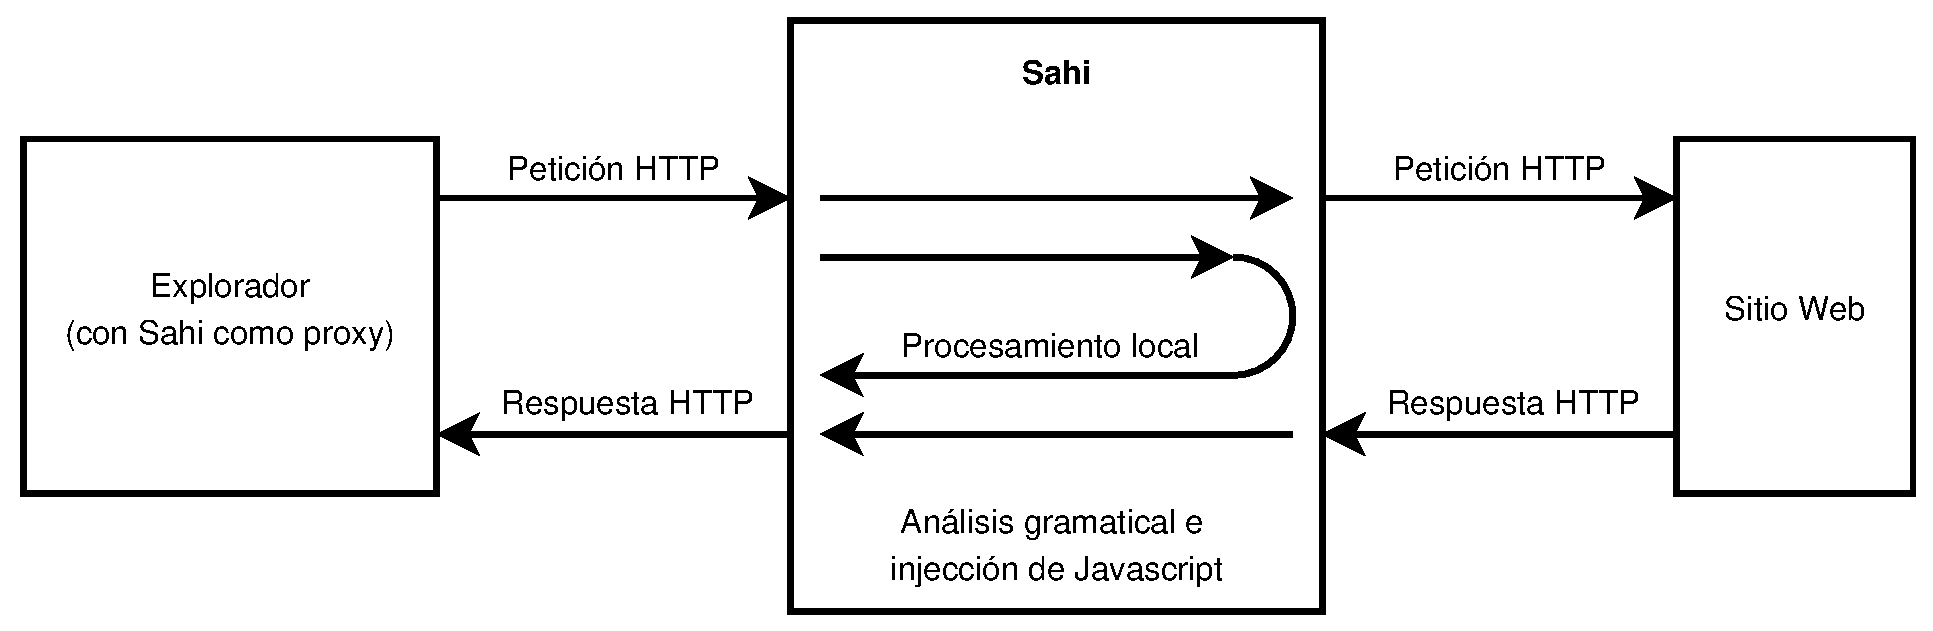
\includegraphics[width=\textwidth]{dia-sahi-arq}
\caption{Diagrama de flujo de Sahi\cite{SahiPro}.}
\label{fig:dia-sahi-arq}
\end{figure}

%\subsubsection{Java IO}
%\subsubsection{Java Enterprise Edition}
%\subsection{Spring}
%\subsubsection{Spring MVC}
%\subsubsection{Spring Security}


\section{Implementación de base de datos}
El sistema AutoSA utiliza una base de datos relacional\footnote{Por confidencialidad no se hace mención específica del nombre y versión del sistema administrador de bases de datos.}(ver sección \ref{sec-bd-r}) para almacenar la información requerida en los casos de uso (ver sección \ref{sec:casos-uso}).\\
La implementación de la base de datos se ve reflejada en las rutinas con sentencias SQL (ver sección \ref{sec-bd-r}) donde se definen los objetos de la base de datos, tales rutinas se separan en dos grupos, las rutinas DDL y las rutinas DML.

%-------------------------------------------------------------------------------
\subsection{Rutinas de definición de datos}
Estas rutinas contienen las sentencias DDL (ver sección \ref{sec-bd-r}) para la creación de tablas, llaves primarias, llaves foráneas, índices y restricciones. En el Código \ref{lst:sql-create-table} se muestra un ejemplo de la creación de la tabla \textit{ordenes\_is}.
\begin{lstlisting}[language=SQL, caption={Sentencia para crear una tabla.}, captionpos=b, label={lst:sql-create-table}]
CREATE TABLE ordenes_is(
   id numeric(20,0) PRIMARY KEY NOT NULL,
   orden numeric(20,0) NOT NULL,
   estatus numeric(2,0) NOT NULL,
   id_sesion_insersion numeric(20,0) NOT NULL,
   id_sesion_estatus numeric(20,0) NOT NULL,
   estatus_sa numeric(2,0),
   estatus_sap numeric(2,0)
);
\end{lstlisting}

La generación de reportes que se menciona en el caso de uso \textbf{Generar reporte} (ver sección \ref{cu-generar-reporte}), utiliza una vista para la definición de la consulta de los datos del reporte (ver Código \ref{lst:sql-create-view}, además se han implementado índices para agilizar tales consultas (ver Código \ref{lst:sql-create-index}).

\begin{lstlisting}[language=SQL, caption={Sentencia para crear una vista.}, captionpos=b, label={lst:sql-create-view}]
CREATE VIEW ordenes_contestadas AS
     SELECT *
       FROM ordenes_is
      WHERE id_sesion_estatus = :sesion
        AND estatus = 3
\end{lstlisting}

\begin{lstlisting}[language=SQL, caption={Sentencia para crear un índice.}, captionpos=b, label={lst:sql-create-index}]
CREATE INDEX ordenes_contetadas_idx ON ordenes_is(id_sesion_estatus, estatus);
\end{lstlisting}

%-------------------------------------------------------------------------------
\subsection{Rutinas de modelado de datos}
Estas rutinas contienen la sentencias DML (ver sección \ref{sec-bd-r}) para insertar la información necesaria para la ejecución del sistema, como son, por ejemplo, los estados posibles de las órdenes de reposición (ver Figura \ref{fig:dia-estados-orden}), en el Código \ref{lst:sql-insert} se muestra un ejemplo de la sentencia DML para insertar un registro.

\begin{lstlisting}[language=SQL, caption={Sentencia insertar un registro.}, captionpos=b, label={lst:sql-insert}]
INSERT INTO cat_estatus_orden (id,nombre) VALUES (1,'NUEVA');
\end{lstlisting}

%================================================================================
%
%================================================================================

\section{Implementación de los componentes}

%-------------------------------------------------------------------------------
\subsection{Agente}
La implementación del componente Agente está escrito en rutinas de Sahi (ver sección \ref{sec-sahi}), primero se exponen los puntos relevantes en la implementación de las rutinas de respuesta y envío de órdenes de reposición para después señalar como se realizar la ejecución mediante la herramienta gráfica de Sahi.

\subsubsection{Rutina para automatizar la respuesta de órdenes de reposición}\label{sec-aut-contestar}
La rutina para automatizar la respuesta de órdenes de reposición refleja el caso de uso  CU-CONTESTAR que se describe en la sección \ref{cu-contestar}. A continuación se muestran las secciones de código más relevantes de la rutina que realizan la ejecución del caso de uso citado así como los subsecuentes (ver diagrama en la Figura \ref{fig:dia-casos-uso}). Los puntos relevantes en la implementación de la rutina son los siguientes:
\begin{enumerate}
	\item Ingresar al Sistema de Abastecimiento, en el Código \ref{lst:sah-session} se muestra la rutina para iniciar sesión en el Sistema de Abastecimiento:
	\begin{enumerate}
		\item Las líneas 1 y 2 se llenan los campos de usuario y contraseña.
		\item La línea 3 se envía el formulario.
		\item La línea 4 redirige a la pantalla con el listado de órdenes de reposición.  
	\end{enumerate}
	\begin{lstlisting}[language=Javascript, caption={Inicio de sesión en el Sistema de Abastecimiento.}, captionpos=b, label={lst:sah-session}]
_setValue(_textbox("Usuario[1]"), $user);
_setValue(_password("Contras[1]"), $pwd);
_click(_submit("Ingresar al Sistema"));
_click(_image("Normal[2]"));
	\end{lstlisting}

	\item Recolectar las órdenes de reposición listadas, el Código \ref{lst:sah-save-news} muestra un resumen de la automatización para guardar el listado de ordenes de reposición (ver caso de uso en la sección \ref{cu-guardar-nueva}):
	\begin{enumerate}
		\item La línea 1 muestra la declaración del ciclo para recorrer el listado de órdenes de reposición.
		\item Las líneas 2 a 4 muestran como se extrae el valor de los datos de una orden de reposición.
		\item Las líneas 5 a 7 muestran la obtención de las URLs para contestar y enviar las órdenes de reposición.
		\item La línea 8 es el almacenamiento de la nueva orden de reposición. 
	\end{enumerate}
	\begin{lstlisting}[language=Javascript, caption={Guardar lista de órdenes de reposición.}, captionpos=b, label={lst:sah-save-news}]
for(var $i = 1 + $errores; $i <= $rowCount; $i++){
	var $contrato = _getText(_table(1).rows[$i].cells[0]);
	var $solicitud = _getText(_table(1).rows[$i].cells[1]);
	var $numorden = _getText(_table(1).rows[$i].cells[2]);
	var $urlcon = "";
	_set($urlcon, _table(1).rows[$i].cells[6].childNodes[0].href);
	var $urlenv = $urlcon.replace("respoOra", "enviaOra");
	var $inserted = $persistence.insertOrden($contrato, $solicitud, $numorden, $expedicion, $almacen, $urlcon, $urlenv, $idSesion);
}
	\end{lstlisting}

	\item Contestar una a una cada orden de reposición, el Código \ref{lst:sah-respond} muestra un resumen de la automatización para contestar una orden de reposición (ver caso de uso en la sección \ref{cu-responder-orden}):
	\begin{enumerate}
		\item Las líneas 1 y 2 muestran como se redirige al explorador a la URL para contestar la orden de reposición.
		\item  Las líneas 3 muestran como se estable un valor en el formulario para contestar la orden de reposición.
		\item La línea 4 realiza el envío del formulario.
		\item La línea 5 manda la actualización de la orden de reposición en la base de datos.
	\end{enumerate}
	\begin{lstlisting}[language=Javascript, caption={Responder orden de reposición.}, captionpos=b, label={lst:sah-respond}]
var $url = $entidad.getUrlCon();
_navigateTo($url);
_setValue(_textbox("Lote"), "SL");
_click(_submit("Agregar Captura"));
$logica.updateCantidad($contrato, $numorden, $cantidad, $idSesion);
	\end{lstlisting}

	\item Enviar las órdenes de reposición contestadas, el Código \ref{lst:sah-send} muestra un resumen de la automatización para envíar una órden de reposición (ver caso de uso en la sección \ref{cu-enviar-orden}):
	\begin{enumerate}
		\item Las líneas 1 y 2 muestran como se redirige al explorador a la URL para enviar la orden de reposición.
		\item La líneas 3 a 6 crea un mapa con los datos de la orden de reposición.
		\item La línea 7 actualiza la orden de reposición en la base de datos. 
	\end{enumerate}
	\begin{lstlisting}[language=Javascript, caption={Enviar orden de reposición.}, captionpos=b, label={lst:sah-send}]
var $url = $entidad.getUrlEnv();
_navigateTo($url);
$mapa = new java.util.LinkedHashMap();
for(var $llave in $orden){
	$mapa.put($llave, $orden[$llave]);
}
$logica.updateOrden($mapa, $idSesion);
	\end{lstlisting}
\end{enumerate}

\subsubsection{Rutina para automatizar la verificación de órdenes de reposición canceladas}
La rutina para automatizar la verificación de órdenes de reposición canceladas refleja el caso de uso  CU-VERIFICAR que se describe en la sección \ref{cu-verificar}, a continuación se muestran las secciones de código más relevantes de la rutina que realizan la ejecución del caso de uso citado así como los subsecuentes (ver diagrama en la Figura \ref{fig:dia-casos-uso}). Los puntos relevantes en la implementación de la rutina son los siguientes:
\begin{enumerate}
	\item Ingresar al Sistema de Abastecimiento, el ingreso al sistema es idéntico a la rutina mostrada en la sección anterior (sección \ref{sec-aut-contestar}).

	\item Establecer los criterios de búsqueda, el Código \ref{lst:sah-search} muestra un resumen de la automatización para:
	\begin{enumerate}
		\item La línea 1 muestra la consulta de las fechas que acotan la búsqueda.
		\item Las líneas 2 a 5 realizan la búsqueda en el Sistema de Abastecimiento.
		\item Las líneas 6 y 7 extraen la información de las órdenes de reposición que muestra el Sistema de Abastecimiento como resultado de la búsqueda.
		\item Las líneas 8 y 9 utilizan el componente \textbf{Lógica de automatización} para actualizar en la base de datos el estado de las órdenes de reposición canceladas.
	\end{enumerate}
	\begin{lstlisting}[language=Javascript, caption={Responder orden de reposición.}, captionpos=b, label={lst:sah-search}]
$dateLimits = $logica.getDateLimits('dd/MM/yyyy');
_setSelected(_select("OrdStt"), "Canceladas");
_setValue(_textbox("OrdFeD"), $dateLimits[0]);
_setValue(_textbox("OrdFeA"), $dateLimits[1]);
_click(_submit(0));
var $html = '';
_set($html, _table(5).innerHTML);
$estado = $logica.getCancelStatus();
$logica.setSaiStatus($html, $estado, $idSesion);
	\end{lstlisting}
\end{enumerate}

\subsubsection{Ejecución de las rutinas de automatización}
La ejecución de las rutinas de sahi corresponden a los casos de uso CU-CONTESTAAR y 
CU-VERIFICAR (ver secciones \ref{cu-contestar} y \ref{cu-verificar} respectivamente), en ambos casos la ejecución es  
dejando la ejecución al usuario por medio de la interfaz gráfica de Sahi:
\begin{itemize}
	\item Iniciar Sahi sobre el explorar de Internet (ver Figura \ref{fig:ss-sahi-dashboard})
	\begin{figure}[h]
	\centering
	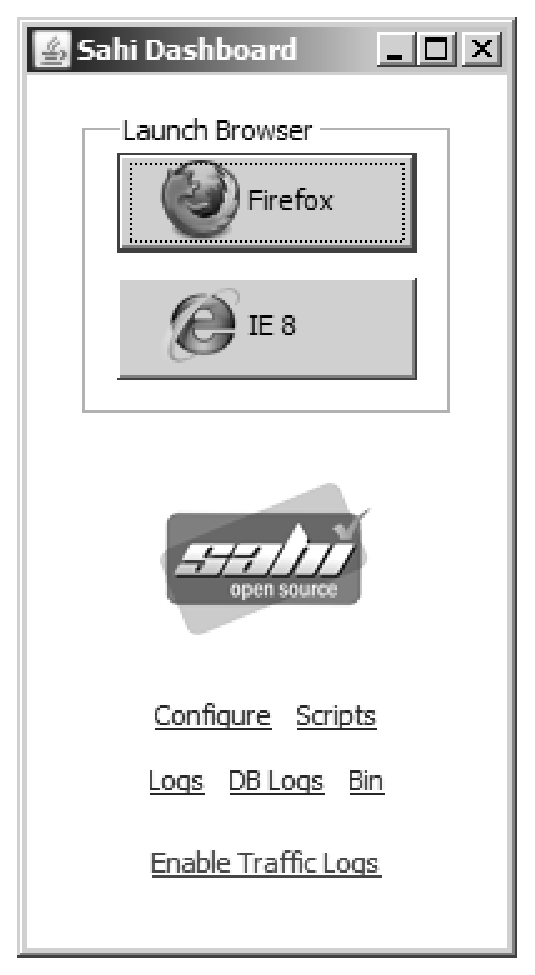
\includegraphics[scale=0.6]{ss-sahi-dashboard}
	\caption{Dashboard de Sahi.}
	\label{fig:ss-sahi-dashboard}
	\end{figure}

	\item Iniciar el controlador de Sahi y hacer los siguientes pasos (ver Figura \ref{fig:ss-sahi-controller}):
	\begin{enumerate}
		\item Seleccionar la rutina automatizada (contestar órdenes de reposición o verificación de órdenes de reposición)
		\item Ingresar la URL del Sistema de Abastecimiento
		\item Iniciar la ejecución.
	\end{enumerate}
	\begin{figure}[h]
	\centering
	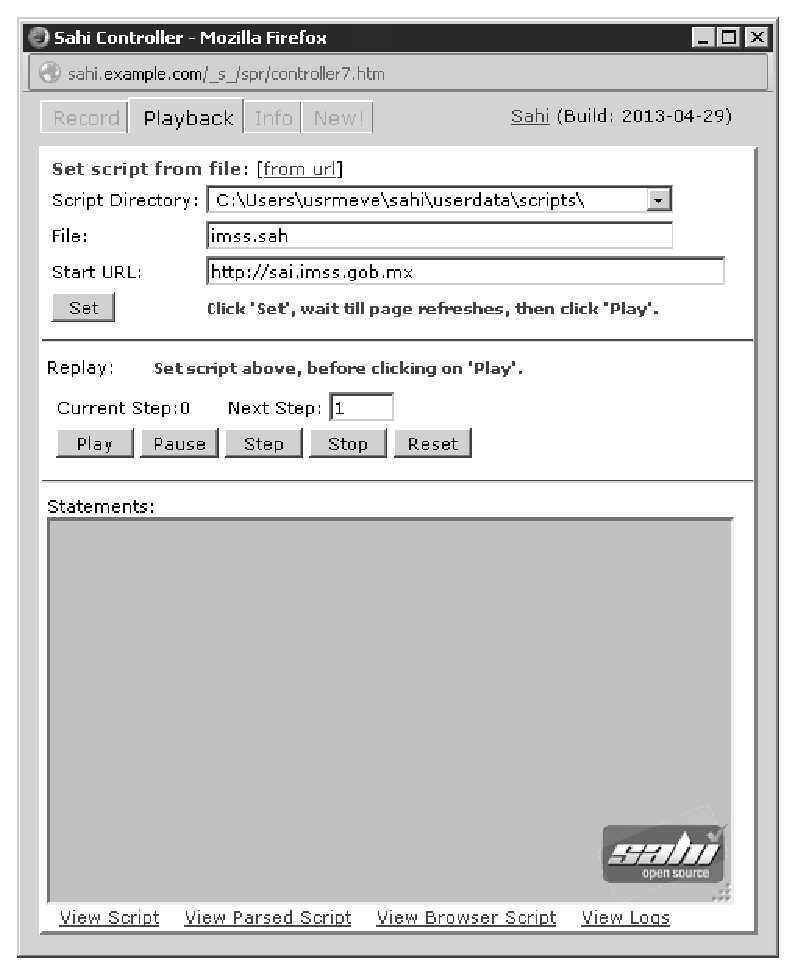
\includegraphics[scale=0.6]{ss-sahi-controller}
	\caption{Controlador de Sahi.}
	\label{fig:ss-sahi-controller}
	\end{figure}
\end{itemize}

%-------------------------------------------------------------------------------
\subsection{Lógica de automatización}
El componente de lógica de automatización provee de la información necesaria a las rutinas automatizadas, la información puede proceder de fuentes diferentes y a cada una se accede de forma diferente:
\begin{enumerate}
 	\item Un archivo en el sistema de archivos del sistema operativo, se obtiene información utilizando el componente \textbf{Sistema de Archivos}.
 	\item Información almacenada en la base de datos, se tiene acceso miente el componente \textbf{Persistencia}.
 	\item Cálculos que corresponde a la lógica de negocio, estos datos se obtienen mediante la aplicación de reglas implementadas dentro del componente \textbf{Lógica de automatización}.
\end{enumerate}
La implementación de este componente ha sido escrita en el lenguaje de programación Java (ver sección \ref{sec-java}).\\
%Dado que la implementación a los datos en el sistema de archivos del sistema operativo y los almacenados en la base de datos son adquiridos mediante otros componentes, únicamente haré mención de la implementación de los datos que se obtienen por medio de reglas de negocio.
A continuación se muestran los puntos relevantes de la implementación de las interfaces mencionadas en la sección \ref{sec-logica-auto}:
\paragraph{\indent Interfaz Respuesta}
\begin{enumerate}
	\item guardar-orden-nueva: la implementación de esta operación (ver Código \ref{lst:la-save-new}) muestra como se delega la aplicación del almacenamiento de una nueva orden de reposición al componente \textbf{Persistencia}.
	\begin{lstlisting}[language=Java, caption={Delegación del almacenamiento de una nueva orden de reposición.}, captionpos=b, label={lst:la-save-new}]
Orden orden = new Orden();
orden.setContrato(contrato);
orden.setSolicitud(Long.parseLong(solicitud));
orden.setOrden(ordenLong);
orden.setFechaExpedicion(fechaExpedicion);
orden.setAlmacenDestino(Long.parseLong(almacenDestino));
orden.setUrlCon(urlCon);
orden.setUrlEnv(urlEnv);
orden.setEstatus(1);
orden.setIdSesionInsersion(idSesion);
orden.setIdSesionEstatus(idSesion);

ordenesDAO.insertOrden(orden);
	\end{lstlisting}

	\item obtener-datos-respuesta: la implementación del cálculo de fechas de fabricación y de caducidad descrita en el caso de uso \textbf{CU-RESPONDER-ORDEN} (ver sección \ref{cu-responder-orden}), Código \ref{lst:la-dates} muestra el método en lenguaje Java:
	\begin{enumerate}
		\item En las líneas 2 a 7 se calcula el año para las fechas de fabricación y de caducidad.
		\item En las líneas 8 a 10 se construyen las fechas de fabricación y de caducidad.
	\end{enumerate}
	\begin{lstlisting}[language=Java, caption={Método para calcular las fechas de fabricación y caducidad.}, captionpos=b, label={lst:la-dates}]
public String[] getFechasFab(){
	Calendar today = GregorianCalendar.getInstance();
	int anho;
	if(Calendar.DECEMBER == today.get(Calendar.MONTH)){
		anho = today.get(Calendar.YEAR) + 1;
	}else{
		anho = today.get(Calendar.YEAR);
	}
	String[] fechas = new String[2];
	fechas[0] = "01/01/" + anho;
	fechas[1] = "31/12/" + anho;
	
	return fechas;
}
	\end{lstlisting}

	\item obtener-acuse-envio: esta operación principalmente obtiene las rutas en el sistema de archivos para la generación del acuse de envío, posteriormente delega la generación del acuse al componente \textbf{Generación de reportes}. En el Código \ref{lst:la-acuse} se muestra el código de Java que realiza los pasos anteriores.
	\begin{enumerate}
		\item La línea 1 estable el nombre del archivo como el número de la orden de reposición.
		\item La línea 2 obtiene la plantilla del acuse de envío para el Instituto de Salud.
		\item La línea 3 obtiene la ruta donde se depositan los archivos auxiliares en la generación del acuse de envío.
		\item Las líneas 4 a 7 construyen la ruta de directorios donde se depositará el acuse de envío.
		\item La línea 8 utiliza el componente \textbf{Generador de Reportes} para la creación del acuse de envío.
	\end{enumerate}
	\begin{lstlisting}[language=Java, caption={Generación del acuse de envío.}, captionpos=b, label={lst:la-acuse}]
String filename = params.get("numorden");
String template = properties.getProperty("is.template.html");
File outhtmldir = new File(properties.getProperty("is.output.dir"), filename + ".html");
SimpleDateFormat sdf = new SimpleDateFormat("yyyy MMMM dd", new Locale("es", "MX"));
String[] date = sdf.format(new Date()).split(" ");
File outputdir = new File(properties.getProperty("is.output.pdf"), String.format(REPORT_DIR_TMPL, date[0], date[1], date[2]));
outputdir.mkdirs();
snapShotService.takeSnapShot(params, filename, template, outhtmldir, outputdir);
	\end{lstlisting}
\end{enumerate}

\paragraph{\indent Interfaz Verificación}
\begin{enumerate}
	\item obtener-rango-fechas-verificar: el Código \ref{lst:la-date-search} muestra el cálculo de las fechas necesarias para el formulario de búsqueda de órdenes de reposición.
	\begin{enumerate}
		\item La línea 5 muestra la obtención de la fecha mayor (día actual).
		\item La líneas 6 y 7 muestran la obtención de la fecha menor (60 días antes de la fecha actual).
	\end{enumerate}
	\begin{lstlisting}[language=Java, caption={Cálculo del rango de fechas para buscar órdenes de reposición canceladas.}, captionpos=b, label={lst:la-date-search}]
DateFormat dateFormat = new SimpleDateFormat(format);
Calendar cal = GregorianCalendar.getInstance();
String[] dates = new String[2];
dates[1] = dateFormat.format(cal.getTime());
cal.add(Calendar.DAY_OF_YEAR, -60);
dates[0] = dateFormat.format(cal.getTime());
	\end{lstlisting}

	\item actualizar-estado-sa: Esta operación realiza la actualización de las órdenes de reposición canceladas, en el Código \ref{lst:la-validate} muestra el código Java.
	\begin{enumerate}
		\item La línea 1 obtiene las órdenes de reposición canceladas del listado de órdenes de reposición encontradas.
		\item La línea 2 actualiza el estado de las órdenes de reposición.
	\end{enumerate}
	\begin{lstlisting}[language=Java, caption={Actualización de órdenes de reposición canceladas.}, captionpos=b, label={lst:la-validate}]
	List<Orden> ordenes = xmlReader.getCancelled(htmlTable);
	persistence.updateSaiStatus(ordenes, status);
	\end{lstlisting}
\end{enumerate}

%-------------------------------------------------------------------------------
\subsection{Persistencia}
La implementación del componente de persistencia se enfoca en dar servicio a los componentes de escritorio y web, por esta razón la implementación se ha dividido en dos partes:
\begin{enumerate}
 	\item Escritorio: la automatización de rutinas, dado que estas rutinas son ejecutadas dentro del ambiente de Sahi (que a su vez está en la plataforma de Java) se utiliza la biblioteca JDBC (ver sección \ref{sec-jdbc}) por economía en recursos físicos del equipo del operador de la farmacéutica.
 	\item Web: generación de reportes, administración de órdenes de reposición, administración de catálogos y operaciones de identificación  de usuarios. Para esta parte se utilizó el marco de trabajo de Spring enfocado a la persistencia, Spring Data (ver sección \ref{sec-spring-jpa}) en conjunción con el marco de trabajo MyBatis (ver sección \ref{sec-mybatis}).
\end{enumerate}
Los siguientes apartados explican la implementación de los servicios para escritorio y web.

\subsubsection{Persistencia para funcionalidades de escritorio}
\paragraph{\indent Interfaz Almacenamiento\\}
Implementación de las operaciones para las rutinas de automatización que requieren almacenar o modificar datos, para simplificar la explicación se mostrarán ejemplos de la manipulación de datos en lugar de mostrar la implementación de cada operación de la interfaz:
\begin{enumerate}
	\item Inserción: la operación de inserción se ocupa en las operaciones \textbf{guardar-nueva} y \textbf{registrar-evento}, la inserción consiste de los siguientes puntos (en el Código \ref{lst:per-insert-order} se muestra la implementación de la operación \textbf{guardar-nueva}):
	\begin{enumerate}
		\item Plantilla de la sentencia SQL, línea 1 del Código \ref{lst:per-insert-order}.
		\item Creación de los objetos de la biblioteca JDBC, línea 4 del Código \ref{lst:per-insert-order}.
		\item Agregar datos específicos de la inserción, líneas 5 a 7 del Código \ref{lst:per-insert-order}.
		\item Ejecución de la sentencia, línea 8 del Código \ref{lst:per-insert-order}.
	\end{enumerate}

	\begin{lstlisting}[language=Java, caption={Inserción de una nueva orden de reposición en la base de datos.}, captionpos=b, label={lst:per-insert-order}]
private static final String INSERT_ORDEN = "INSERT INTO ordenes(contrato, solicitud, orden, fecha_expedicion, almacen_destino, url_con, url_env, estatus, id_sesion_insersion, id_sesion_estatus, fecha_estatus) VALUES(?, ?, ?, ?, ?, ?, ?, 1, ?, ?, CURRENT_TIMESTAMP)";

public void insertOrden(Orden orden) throws SQLException{
    try(PreparedStatement pst = conn.prepareStatement(INSERT_ORDEN)){
	    pst.setString(1, orden.getContrato());
	    ...
	    pst.setLong(9, orden.getIdSesionInsersion());
	    pst.executeUpdate();
	}
}
	\end{lstlisting}

	\item Actualización: la actualización de datos es utilizada por las operaciones \textbf{cambiar-estado}, \textbf{guardar-respuesta}, \textbf{guardar-folio-acuse} y \textbf{actualizar-estado-sa}, la actualización consiste de los siguientes puntos (en el Código \ref{lst:per-update-status} se muestra la implementación de la operación \textbf{cambiar-estado}):
	\begin{enumerate}
		\item Plantilla de la sentencia SQL, línea 1 del Código \ref{lst:per-update-status}.
		\item Creación de los objetos de la biblioteca JDBC, línea 4 del Código \ref{lst:per-update-status}.
		\item Agregar datos de la actualización, líneas 5 a 8 del Código \ref{lst:per-update-status}.
		\item Ejecución de la sentencia, línea 9 del Código \ref{lst:per-update-status}.
	\end{enumerate}

	\begin{lstlisting}[language=Java, caption={Actualización del estado de una orden de reposición.}, captionpos=b, label={lst:per-update-status}]
private static final String UPDATE_STATUS = "UPDATE ordenes SET estatus = ?, fecha_estatus = CURRENT_TIMESTAMP, id_sesion_estatus = ? WHERE contrato = ? AND orden = ?";

private void updateEstatus(Orden orden) throws SQLException{
	try(PreparedStatement pst = conn.prepareStatement(UPDATE_STATUS)){
		pst.setInt(1, orden.getEstatus());
		pst.setLong(2, orden.getIdSesionEstatus());
		pst.setString(3, orden.getContrato());
		pst.setLong(4, orden.getOrden());
		pst.executeUpdate();
	}
}
	\end{lstlisting}
\end{enumerate}

\paragraph{\indent Interfaz Lectura\\}
Implementación de las operaciones para las rutinas de automatización que tienen como objetivo la obtención de datos, esto no quiere decir que durante el llamado de estas operaciones no se modifiquen datos.
Dado que la obtención de los datos se convierte a objetos del dominio del proyecto AutoSA, se ha implementado una solución basada en los patrones de diseño Strategy (ver Apéndice \ref{sec-strategy}) y Singleton (ver Apéndice \ref{sec-singleton}). \\
En la Figura \ref{fig:dia-class-mapper} se el diagrama de clases de la solución:
\begin{figure}[h]
	\centering
	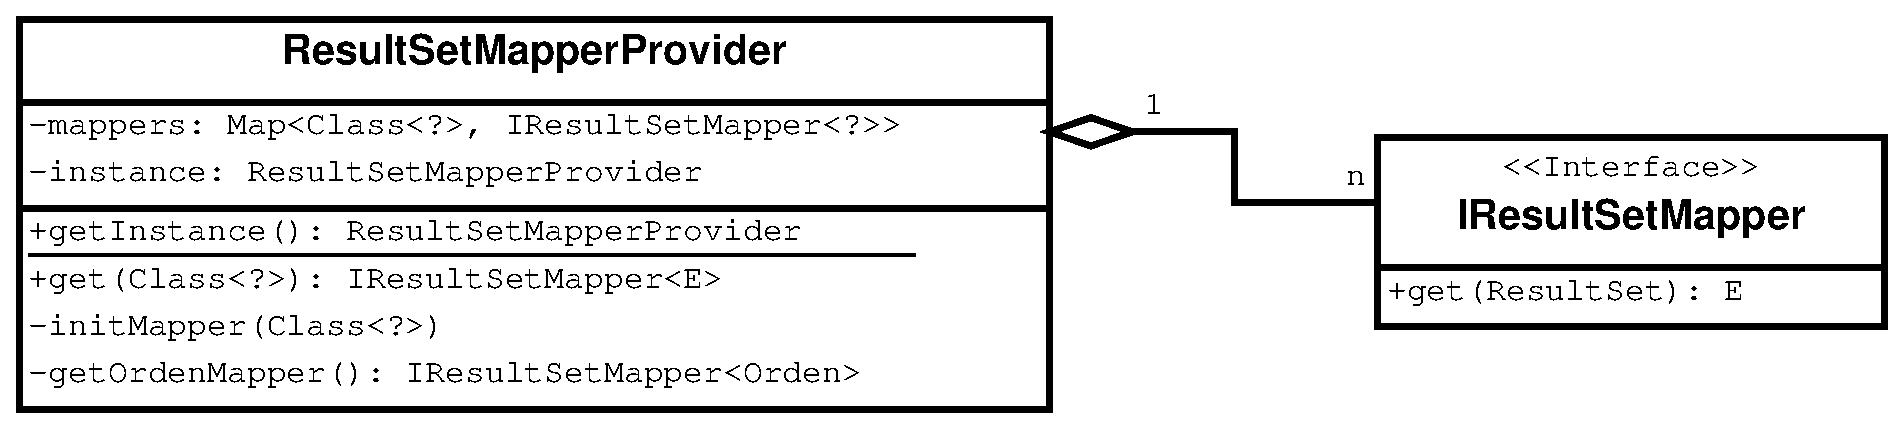
\includegraphics[width=\textwidth]{dia-class-mapper}
	\caption{Diagrama de clase de ResultSetMapperProvider.}
	\label{fig:dia-class-mapper}
\end{figure}

La clase \textbf{IResultSetMapper} tiene como función la conversión de la información obtenida por la biblioteca JDBC de la base de datos a objetos del dominio del proyecto AutoSA. El Código \ref{lst:per-i-rs-mapper} muestra la definición de la interfaz de Java.
	\begin{lstlisting}[language=Java, caption={Interfaz IResultSetMapper.}, captionpos=b, label={lst:per-i-rs-mapper}]
public interface IResultSetMapper<E>{
	E get(ResultSet resultSet) throws SQLException;
}
	\end{lstlisting}

La clase \textbf{ResultSetMapperProvider} es la encargada de la construcción y administración de las clases del tipo \textbf{IResultSetMapper}.\\
El Código \ref{lst:per-class-mapper-provider} muestra la declaración del la clase \textbf{ResultSetMapperProvider} donde se observa el uso del patrón de diseño Singleton:
\begin{enumerate}
	\item Línea 3, instancia privada de la clase.
	\item Línea 5, constructor de clase privado.
	\item Línea 9, método para obtener la instancia de clase.
\end{enumerate}

\begin{lstlisting}[language=Java, caption={Clase ResultSetMapperProvider con patrón de diseño Singleton.}, captionpos=b, label={lst:per-class-mapper-provider}]
public class ResultSetMapperProvider{
	private final Map<Class<?>, IResultSetMapper<?>> mappers;
	private static ResultSetMapperProvider instance;
	
	private ResultSetMapperProvider(){
		mappers = new LinkedHashMap<Class<?>, IResultSetMapper<?>>();
	}
	
	public static ResultSetMapperProvider getInstance(){
		if(instance == null){
			instance = new ResultSetMapperProvider();
		}
		return instance;
	}

	public <E> IResultSetMapper<E> get(Class<?> beanType){...}
	private void initMapper(Class<?> beanType){...}
	private IResultSetMapper<Orden> getOrdenMapper(){...}
}
\end{lstlisting}

La clase \textbf{ResultSetMapperProvider} realiza la construcción de los objetos del tipo \textbf{IResultSetMapper} como se muestra en el Código \ref{lst:per-get-orden-mapper}:
\begin{lstlisting}[language=Java, caption={}, captionpos=b, label={lst:per-get-orden-mapper}]
private IResultSetMapper<Orden> getOrdenMapper(){
	return new IResultSetMapper<Orden>(){
		public Orden get(ResultSet rs) throws SQLException{
			Orden orden = new Orden();
			orden.setId(rs.getLong("id"));
			...
			return orden;
		}
	};
}
\end{lstlisting}

La clase \textbf{ResultSetMapperProvider} da acceso a las instancias de tipo \textbf{IResultSetMapper} mediante el método \textbf{get} como se muestra en las líneas 1 a 6 del Código \ref{lst:per-get-rs-mapper}, si no se encuentra una instancia para la clase solicitada, entonces se crea como se muestra en las líneas 2 a 4 y 8 a 20 del Código \ref{lst:per-get-rs-mapper}
\begin{lstlisting}[language=Java, caption={Obtención de instancias de IResultSetMapper.}, captionpos=b, label={lst:per-get-rs-mapper}]
public <E> IResultSetMapper<E> get(Class<?> beanType){
	if(!mappers.containsKey(beanType)){
		initMapper(beanType);
	}
	return (IResultSetMapper<E>)mappers.get(beanType);
}

private void initMapper(Class<?> beanType){
	if(Orden.class.equals(beanType)){
		mappers.put(beanType, getOrdenMapper());
	}else if(OrdenPemex.class.equals(beanType)){
		mappers.put(beanType, getPemexMapper());
	}else if(ProductoPemex.class.equals(beanType)){
		mappers.put(beanType, getProductoPemexMapper());
	}else if(Sesion.class.equals(beanType)){
		mappers.put(beanType, getSesionMapper());
	}
}
\end{lstlisting}

La solución anterior lleva a la implementación de las operaciones de la interfaz ``Lectura'':
\begin{enumerate}
	\item \textbf{siguiente-orden-contestar}, \textbf{siguiente-orden-enviar} y \textbf{obtener-datos-acuse}: todas las operaciones de lectura siguen los mismos pasos (en el Código \ref{lst:per-next-orden} se muestra la implementación de la operación \textbf{siguiente-orden-contestar}):
	\begin{enumerate}
		\item Plantilla de la sentencia SQL, línea 1 del Código \ref{lst:per-next-orden}.
		\item Creación de los objetos de la biblioteca JDBC, línea 4 del Código \ref{lst:per-next-orden}.
		\item Realizar la consulta a la base de datos, línea 6 del Código \ref{lst:per-next-orden}.
		\item Lectura del resultado de la consulta, líneas 7 a 9 del Código \ref{lst:per-next-orden}.
	\end{enumerate}

	\begin{lstlisting}[language=Java, caption={Lectura de una orden de reposición desde la base de datos.}, captionpos=b, label={lst:per-next-orden}]
private static final String NEXT_TO_MANAGE = "SELECT * FROM ordenes WHERE estatus = ? ORDER BY fecha_insersion LIMIT 1";

public Orden getNextOrden(Integer estatus) throws SQLException{
	try(PreparedStatement pst = conn.prepareStatement(NEXT_TO_MANAGE)){
		pst.setInt(1, estatus);
		try(ResultSet rs = pst.executeQuery()){
    		if(rs.next()){
    			IResultSetMapper<Orden> mapper = ResultSetMapperProvider.getInstance().get(Orden.class);
    			return mapper.get(rs);
    		}
		}
	}
	return null;
}
	\end{lstlisting}
\end{enumerate}

\subsubsection{Persistencia para funcionalidades Web}
La interfaz del componente Persistencia dedicado a las funcionalidades ofrecidas mediante la interfaz web utiliza MyBatis cuya implementación sigue los pasos mencionados en la sección \ref{sec-mybatis}.\\
\indent 1. En el Código \ref{lst:per-batis-config} se muestra la configuración del objeto \textbf{SqlSessionFactoryBean}: 
\begin{enumerate}
	\item Línea 1, habilitar contexto para transacciones.
	\item Línea 2, crear los objetos para manejar la persistencia.
	\item Línea 3, lectura de las interfaces para crear los objetos de persistencia.
\end{enumerate}
\begin{lstlisting}[language=XML, caption={Configuración de MyBatis con Spring.}, captionpos=b, label={lst:per-batis-config}]
<tx:annotation-driven />
<bean id="sqlSessionFactory" class="org.mybatis.spring.SqlSessionFactoryBean">
	<property name="dataSource" ref="dataSource" />
	<property name="mapperLocations" value="classpath:com/surtimiento/persistence/dao/*.xml" />
</bean>
<mybatis:scan base-package="com.surtimiento.persistence.dao"/>
\end{lstlisting}

\indent 2. El Código \ref{lst:per-batis-user} muestra la configuración para el manejo de usuarios de la interfaz web:
\begin{enumerate}
	\item Relación entre tabla de roles y clase Rol.
	\item Relación entre tabla de usuarios y clase de Usuario.
	\item Consulta SQL para obtener un usuario.
\end{enumerate}
\begin{lstlisting}[language=XML, caption={Definición de relación de MyBatis.}, label={
lst:per-batis-user}]
<mapper namespace="com.meve.surtimiento.persistence.dao.IDomainUser">
  <resultMap id="rol" type="com.meve.surtimiento.domian.RolDomain" autoMapping="true">
    <id property="rol" column="rol"/>
  </resultMap>
  <resultMap id="usuario" type="com.meve.surtimiento.domian.UsuarioDomain" autoMapping="true">
    <id property="usuario" column="usuario"/>
    <collection property="roles" resultMap="rol" javaType="ArrayList"/>
  </resultMap>
  <select id="getUsuario" resultMap="usuario" useCache="false">
    SELECT u.*, r.*
      FROM usuarios u, roles_domain r, usuarios_roles ur
     WHERE u.usuario = ur.usuario AND r.rol = ur.rol AND u.usuario = #{0};
  </select>
</mapper>
\end{lstlisting}

\indent 3. Por último se el Código \ref{lst:per-batis-user-interface} muestra la interfaz de Java para utilizar las consultas del paso anterior.
\begin{lstlisting}[language=Java, caption={Interfaz de Java para la fábrica de MyBatis.}, captionpos=b, label={lst:per-batis-user-interface}]
public interface IDomainUser{
	UsuarioDomain getUsuario(String name);
}
\end{lstlisting}

%-------------------------------------------------------------------------------
\subsection{Sistema de archivos}
	\paragraph{Configuración\\}
		\textbf{obtener-propiedad}
	\paragraph{Almacenamiento\\}
		\textbf{guardar-archivo}

%
%\subsection{Generador de reportes}
%
%\textcolor{blue}{En el diseño debe agregarse un diagrama del funcionamiento de reportes: seleccionar templates... agregar patrones de diseño}\\
%\subsection{Motor de plantillas}
%\textcolor{blue}{aquí platico de volicity y como funciona el motor}\\
%\textcolor{blue}{aquí va la configuración}\\
%\textcolor{blue}{tipos de reporte}
%
%	\paragraph{Acuse\\}
%		\textbf{generar-acuse-envio}
%	\paragraph{Generación\\}
% 		\textbf{generar-reporte-ordenes}
%
%
%\subsection{Portal Web}
%\textcolor{blue}{Las secciones de esta parte serán presentadas por capas desde datos hasta la vista}\\
%\textcolor{blue}{Presentar el patron MVC}\\
%\subsection{Acceso}
%\textcolor{blue}{Spring security}\\
%\textcolor{blue}{Cifrado de contraseña}\\
%\subsection{Generación de reportes}
%\subsection{Búsqueda}
%
%\subsection{Administración de catálogos}
%
%\subsection{Visualización de órden de reposición}
%
%\subsection{Edición de órden de reposición}









%\section{Implmenetación de genración de reportes}

%\section{Implementación de automatización para SA}
%\subsection{Bibliotecas para las rutinas de automatización}
%\subsection{Rutinas de automatización}




